\documentclass[12pt,]{article}
\usepackage{lmodern}
\usepackage{amssymb,amsmath}
\usepackage{ifxetex,ifluatex}
\usepackage{fixltx2e} % provides \textsubscript
\ifnum 0\ifxetex 1\fi\ifluatex 1\fi=0 % if pdftex
  \usepackage[T1]{fontenc}
  \usepackage[utf8]{inputenc}
\else % if luatex or xelatex
  \ifxetex
    \usepackage{mathspec}
    \usepackage{xltxtra,xunicode}
  \else
    \usepackage{fontspec}
  \fi
  \defaultfontfeatures{Mapping=tex-text,Scale=MatchLowercase}
  \newcommand{\euro}{€}
\fi
% use upquote if available, for straight quotes in verbatim environments
\IfFileExists{upquote.sty}{\usepackage{upquote}}{}
% use microtype if available
\IfFileExists{microtype.sty}{%
\usepackage{microtype}
\UseMicrotypeSet[protrusion]{basicmath} % disable protrusion for tt fonts
}{}
\usepackage[margin=1in]{geometry}
\usepackage{graphicx}
\makeatletter
\def\maxwidth{\ifdim\Gin@nat@width>\linewidth\linewidth\else\Gin@nat@width\fi}
\def\maxheight{\ifdim\Gin@nat@height>\textheight\textheight\else\Gin@nat@height\fi}
\makeatother
% Scale images if necessary, so that they will not overflow the page
% margins by default, and it is still possible to overwrite the defaults
% using explicit options in \includegraphics[width, height, ...]{}
\setkeys{Gin}{width=\maxwidth,height=\maxheight,keepaspectratio}
\ifxetex
  \usepackage[setpagesize=false, % page size defined by xetex
              unicode=false, % unicode breaks when used with xetex
              xetex]{hyperref}
\else
  \usepackage[unicode=true]{hyperref}
\fi
\hypersetup{breaklinks=true,
            bookmarks=true,
            pdfauthor={},
            pdftitle={},
            colorlinks=true,
            citecolor=blue,
            urlcolor=black,
            linkcolor=black,
            pdfborder={0 0 0}}
\urlstyle{same}  % don't use monospace font for urls
\setlength{\parindent}{0pt}
\setlength{\parskip}{6pt plus 2pt minus 1pt}
\setlength{\emergencystretch}{3em}  % prevent overfull lines
\setcounter{secnumdepth}{0}

%%% Use protect on footnotes to avoid problems with footnotes in titles
\let\rmarkdownfootnote\footnote%
\def\footnote{\protect\rmarkdownfootnote}

%%% Change title format to be more compact
\usepackage{titling}

% Create subtitle command for use in maketitle
\newcommand{\subtitle}[1]{
  \posttitle{
    \begin{center}\large#1\end{center}
    }
}

\setlength{\droptitle}{-2em}
  \title{}
  \pretitle{\vspace{\droptitle}}
  \posttitle{}
  \author{}
  \preauthor{}\postauthor{}
  \date{}
  \predate{}\postdate{}

\usepackage{lineno}
\linenumbers
\usepackage{setspace}
\usepackage{sectsty}
\doublespacing
\usepackage{todonotes}
\usepackage[document]{ragged2e}
\usepackage{times}
\usepackage{enumitem}
\usepackage{color, soul}


\begin{document}

\maketitle


\textsf{\LARGE{\textbf{Do we need demographic data to forecast plant population dynamics?}}}

\renewcommand*{\thefootnote}{\fnsymbol{footnote}}

\vspace{1em}

\textsf{\normalsize{\textbf{Andrew T. Tredennick\textsuperscript{1}\footnote{Corresponding author: E-mail: atredenn@gmail.com}, Mevin B. Hooten\textsuperscript{2,3,4}, and Peter B. Adler\textsuperscript{1}}}}

\vspace{1em}

\textsf{\textit{\footnotesize{\textsuperscript{1}Department of Wildland Resources and the Ecology Center, 5230 Old Main Hill, Utah State University, Logan, Utah 84322, USA; \textsuperscript{2}U.S. Geological Survey, Colorado Cooperative Fish and Wildlife Research Unit, Fort Collins, CO 80523, USA; \textsuperscript{3}Department of Fish, Wildlife, and Conservation Biology, Colorado State University, Fort Collins, CO 80523 USA}; \textsuperscript{4}Department of Statistics, Colorado State University, Fort Collins, CO 80523 USA}}

\textbf{Running head:} Demographic data and population forecasting

\textbf{Word count:} 6845 (including reference section)

\textbf{Corresponding author:}\\Andrew Tredennick
(\href{mailto:atredenn@gmail.com}{\nolinkurl{atredenn@gmail.com}})\\Department
of Wildland Resources and the Ecology Center\\5230 Old Main Hill\\Utah
State University\\Logan, Utah 84322, USA

Last compile: \today

\allsectionsfont{\normalfont\sffamily\bfseries}
\renewcommand*{\thefootnote}{\arabic{footnote}} \setcounter{footnote}{0}

\rule{\textwidth}{1pt}

\subsection{Summary}\label{summary}

\begin{enumerate}[label=\textbf{\arabic*}]
        \item Rapid environmental change has generated growing interest in forecasts of future population trajectories. Traditional population models built with detailed demographic observations from one study site can address the impacts of environmental change at particular locations, but are difficult to scale up to the landscape and regional scales relevant to management decisions. An alternative is to build models using population-level data that are much easier to collect than individual-level data over broad spatial scales. However, it is unknown whether models built using population-level data adequately capture the effects of density-dependence and environmental forcing that are necessary to generate skillful forecasts.
        \item Here, we test the consequences of aggregating individual responses when forecasting the population states \textcolor{blue}{(percent cover)} and trajectories of four perennial grass species in a semi-arid grassland in Montana, USA. We parameterized two population models for each species, one based on individual-level data (survival, growth and recruitment) and one on population-level data (percent cover), and compared their forecasting \textcolor{blue}{accuracy} and forecast horizons with and without the inclusion of climate covariates. For both models, we used Bayesian ridge regression to weight the influence of climate covariates for optimal prediction. 
        \item In the absence of climate effects, we found no significant difference between the forecast \textcolor{blue}{accuracy} of models based on individual-level data and models based on population-level data. Climate effects were weak, but increased forecast \textcolor{blue}{accuracy} for two species. Increases in \textcolor{blue}{accuracy} with climate covariates were similar between model types.
        \item In our case study, percent cover models generated forecasts as \textcolor{blue}{accurate} as those from a demographic model. For the goal of forecasting, models based on aggregated individual-level data may offer a practical alternative to data-intensive demographic models. Long time series of percent cover data already exist for many plant species. Modelers should exploit these data to predict the impacts of environmental change.
    \end{enumerate}

\textsf{\textbf{Key-words:}} forecasting, climate change, grassland,
integral projection model, population model, statistical regularization,
ridge regression

\subsection{Introduction}\label{introduction}

Perhaps the greatest challenge for ecology in the 21st century is to
forecast the impacts of environmental change (Clark et al. 2001, Petchey
et al. 2015). Forecasts require sophisticated modeling approaches that
fully account for uncertainty and variability in both ecological process
and model parameters (Luo et al. 2011, but see Perretti et al. 2013).
The increasing statistical sophistication of population models (Rees and
Ellner 2009) makes them promising tools for predicting the impacts of
environmental change on species persistence and abundance. But
reconciling the scales at which population models are parameterized with
the scales at which environmental changes play out remains a challenge
(Clark et al. 2010, 2012, Freckleton et al. 2011, Queenborough et al.
2011). Most population models are built using demographic data from a
single study site because tracking the fates of individuals is so
difficult. The resulting models cannot be applied to the landscape and
regional scales relevant to decision-making without information about
how the estimated parameters respond to spatial variation in biotic and
abiotic drivers (S{æ}ther et al. 2007). The limited spatial extent of
individual-level demographic datasets constrains our ability to use
population models to address applied questions about the consequences of
climate change.

Aggregate measures of population status, rather than individual
performance, offer an intriguing alternative for modeling populations
(Clark and Bj{ø}rnstad 2004, Freckleton et al. 2011). Population-level
data cannot provide inference about demographic mechanisms, but might be
sufficient for modeling future population states, especially because
population-level data, such as plant percent cover, are feasible to
collect across broad spatial extents (e.g., Queenborough et al. 2011).
The choice between individual and population-level data involves a
difficult trade-off: while individual-level data are necessary for
mechanistic models, population-level data enable models that can be
applied over greater spatial and temporal extents. An open question is
how much forecasting skill is lost when we build models based on
population rather than individual-level data.

To date, most empirical population modelers have relied on
individual-level data, with few attempts to capitalize on
population-level measures. An important exception was an effort by
Taylor and Hastings (2004) to model the population growth rate of an
invasive species to identify the best strategies for invasion control.
They used a ``density-structured'' model where the state variable is a
discrete density state rather than a continuous density measure. Such
models do not require individual-level demographic data and can
adequately describe population dynamics. Building on Taylor and Hastings
(2004), Freckleton et al. (2011) showed that density-structured models
compare well to continuous models in theory, and Queenborough et al.
(2011) provide empirical evidence that density-structured models are
capable of reproducing population dynamics at landscape spatial scales,
even if some precision is lost when compared to fully continuous models.
However, previous tests of density-structured population models have yet
to assess their ability to forecast out-of-sample observations, and they
have not included environmental covariates, which are necessary to
forecast population responses to climate change.

Addressing climate change questions with models fit to population-level
data is potentially problematic. Population growth (or decline) is the
outcome of demographic processes such as survival, growth, and
recruitment that occur at the level of individual plants. Climate can
affect each demographic process in unique, potentially opposing, ways
(Dalgleish et al. 2011). These unique climate responses may be difficult
to resolve in statistical models based on population-level data where
demographic processes are not identifiable. Futhermore, models based on
aggregated data may reflect short-term effects of one vital rate more
than others whose importance may only emerge over the long-term. For
example, a one-year change in a plant species' cover or biomass might
reflect individual growth or shrinkage, whereas the long-term trajectory
of the population might be more influenced by recruitment. The same is
true for density dependence: intraspecific density depedence may act
most strongly on vital rates, like recruitment, that are difficult to
identify from population-level data. If density dependence and/or
important climate effects are missed because of the aggregation inherent
in population-level data, then population models built with such data
will make uninformative or unreliable forecasts.

We compared the forecasting skill
\textcolor{blue}{(accuracy and precision)} of statistical and population
models based on aggregated, population-level data with the skill of
models based on individual-level data. We used a demographic dataset
that tracks the fates of individual plants from four species over 14
years to build two kinds of single-species population models,
traditional models using individual growth, survival, and recruitment
data and alternative models based on population-level (basal cover)
data. We simulated from the models to answer two questions motivated by
the fact that the effects of intraspecific competition (density
dependence) and interannual weather variability act at the level of the
individual (Clark et al. 2011). First, can population models fit using
aggregated individual-level data (percent cover) adequately capture
density dependence to produce forecasts as skillful as those from models
fit to demographic data? Second, can population models fit using
aggregated data adequately capture the influence of climate on
population growth and, in turn, produce forecasts as skillful as those
from models fit to demographic data?

\subsection{Materials and Methods}\label{materials-and-methods}

\subsubsection{Overview of analysis}\label{overview-of-analysis}

\textcolor{blue}{We used two types of data: individual-level data and percent cover data.
Using the individual-level data, we fit three vital rate regressions (survival, growth, and rectruitment) to build an Integral Projection Model (IPM) for simulating the plant populations.
Using the percent cover data we fit a simple, Gompertz population growth model, which we refer to as a quadrat-based model (QBM).
For both model types (IPM and QBM), we fit and simulate versions of the model with and without climate covariates.
We used Bayesian ridge regression to weight the importance of each climate covariate.
We then performed cross-validation to assess each model's ability to predict out-of-sample data.
We compared the forecast accuracy ($\rho$, correlation between observations and predictions) and mean absolute error (MAE) between the IPM and the QBM to test our expectation that the IPM should outperform the QBM.
Lastly, we use in-sample forecasts to quantify each model's forecast horizon}
(Petchey et al. 2015).

\subsubsection{Study site and data}\label{study-site-and-data}

Our demographic data were obtained from a northern mixed grass prairie
at the Fort Keogh Livestock and Range Research Laboratory near Miles
City, Montana, USA (\(46^{\circ}\) 19' N, \(105^{\circ}\) 48' W). The
dataset is available on Ecological Archives\footnote{\url{http://esapubs.org/archive/ecol/E092/143/}}
(Anderson et al. 2011), and interested readers should refer to the
metadata for a complete description. The site is 800 m above sea level
and mean annual precipitation (1878-2009) is 334 mm, with most annual
precipitation falling from April through September. The community is
grass-dominated, and we focused on the four most abundant grass species:
\emph{Bouteloua gracilis} (BOGR), \emph{Hesperostipa comata} (HECO),
\emph{Pascopyrum smithii} (PASM), and \emph{Poa secunda} (POSE) (Fig. 1
and Table 1). \emph{B. gracilis} is a warm-season perennial grass,
whereas \emph{H. comata}, \emph{P. smithii}, and \emph{Poa secunda} are
cool-season perennial grasses. The growing season begins in early spring
(typically in April) and lasts through mid-summer (typically in June).

From 1932 to 1945, individual plants were identified and mapped annually
in 44 1-\(\text{m}^2\) quadrats using a pantograph. The quadrats were
distributed among six pastures, each assigned a grazing treatment of
light (1.24 ha/animal unit month), moderate (0.92 ha/aum), and heavy
(0.76 ha/aum) stocking rates (two pastures per treatment). In this
analysis, we accounted for potential differences among the grazing
treatments, but do not focus on grazing\(\times\)climate interactions.
The annual maps of the quadrats were digitized and the fates of
individual plants tracked and extracted using a computer program
(Lauenroth and Adler 2008, Chu et al. 2014). The permanent quadrats have
not been relocated, but their distribution in six different pastures
implies that the data represent a broad spatial distribution for the
study area. Daily climate data are available for the duration of the
data collection period (1932 - 1945) from the Miles City airport, Wiley
Field, 9 km from the study site.

We modeled each grass population based on two levels of data: individual
and quadrat. The individual data are the ``raw'' data. For the
quadrat-level data, we summed individual basal cover for each quadrat by
species. This is equivalent to a near-perfect census of quadrat percent
cover because measurement error at the individual-level is small (Chu
and Adler 2015). Based on these two datasets of 13 year-to-year
transitions, we can compare population models built using
individual-level data and aggregated, quadrat-level data. At the
individual level, we explicitly model three vital rates: growth,
survival, and recruitment. At the quadrat level, we model population
growth as change in percent cover of quadrats with non-zero cover in
year \emph{t} and in year \emph{t-1}, ignoring within-quadrat
extirpation and colonization events because they are very rare in our
time series (\(N=16\) and \(N=13\), respectively, across all species).
Sample sizes for each species and vital rate model are shown in Table 1.

All R code and data necessary to reproduce our analysis is archived on
GitHub as release v1.0\footnote{\emph{Note to reviewers}: so that v1.0
  will be associated with the published version of the manuscript, we
  have released v0.2 to be associated with this review version.}
(\url{http://github.com/atredennick/MicroMesoForecast/releases}). We
have also deposited the v1.0 release on Dryad (\emph{link here after
acceptance}).

\subsubsection{Statistical models of vital
rates}\label{statistical-models-of-vital-rates}

At both levels of inference (individual and quadrat), the building
blocks of our population models are vital rate regressions. For
individual-level data, we fit regressions for survival, growth, and
recruitment for each species. At the quadrat-level, we fit a single
regression model for population growth. We describe the statistical
models separately because they required different approaches. For both
model types, we fit vital rate models with and without climate
covariates. Models with climate effects contain five climate covariates
that we chose \emph{a priori} based on previous model selection efforts
using these data (Chu et al. 2016) and expert advice (Lance Vermeire,
\emph{personal communication}): ``water year'' precipitation at
\emph{t}-2 (lagppt); April through June precipitation at \emph{t}-1 and
\emph{t} (ppt1 and ppt2, respectively) and April through June
temperature at \emph{t}-1 and \emph{t} (TmeanSpr1 and TmeanSpr2,
respectively), where \emph{t}-1 to \emph{t} is the transition of
interest. We also include interactions among same-year climate
covariates (e.g., ppt1 \(\times\) TmeansSpr1), resulting in a total of
seven climate covariates.

We fit all models using a hierarchical Bayesian approach. We focus on
the main process and the model likelihood in what follows (full model
descriptions are in the Supporting Information). For the likelihood
models, \(\textbf{y}^X\) is always the relevant vector of observations
for vital rate \emph{X} (\emph{X} = \emph{S}, \emph{G}, \emph{R}, or
\emph{P} for survival, growth, recruitment, or population growth). For
example, \(\textbf{y}^S\) is a vector of 0s and 1s indicating whether a
genet survives from \emph{t} to \emph{t+1}, or not, for all observation
years and quadrats. All model parameters are species-specific, but we
omit subscripts for species in model descriptions below to reduce visual
clutter. For brevity, we only describe models with climate covariates
included, but models without climate covariates are simply the models
described below with the climate effects removed.

\paragraph{Vital rate models at the individual
level}\label{vital-rate-models-at-the-individual-level}

We used logistic regression to model the probability that genet \emph{i}
in quadrat \emph{q} survives from time \emph{t} to \emph{t}+1
(\(s_{i,q,t}\)):

\vspace{-3em}\begin{align}
y_{i,q,t}^{S} &\sim \text{Bernoulli}(s_{i,q,t}), \\
\text{logit}(s_{i,q,t}) &= \beta_{0,t} + \beta_{s,t}x_{i,q,t} + \beta_{Q,q} + \textbf{z}'_t \boldsymbol{\beta}_c + \beta_{d,1} w_{i,t} + \beta_{d,2} (x_{i,q,t}w_{i,q,t}),
\end{align}\vspace{-3em}

where \(x_{i,q,t}\) is the log of genet \emph{i} basal area at time
\emph{t}, \(\beta_{0,t}\) is a year specific intercept, \(\beta_{Q,q}\)
is the random effect of the \emph{q}th quadrat to account for spatial
location, \(\beta_{s,t}\) is the year-specific slope parameter for size,
\textbf{z} is a vector of \emph{p} climate covariates specific to year
\emph{t}, \(\boldsymbol{\beta}_c\) is a vector of fixed climate effects
of length \emph{p}, \(\beta_{d,1}\) is the effect of intraspecific
crowding experienced by the focal genet at time \emph{t}
(\(w_{i,q,t}\)), and \(\beta_{d,2}\) is a size by crowding
(\(x_{i,q,t}w_{i,q,t}\)) interaction effect.

We follow the approach of Chu and Adler (2015) to estimate crowding,
assuming that the crowding experienced by a focal genet depends on
distance to each neighbor genet and the neighbor's size, \emph{u}:

\begin{equation}
w_{i,q,t} = \sum_k e^{-\delta d_{ik,q,t}^{2}}u_{k,q,t}.
\end{equation}

In equation 3, \(w_{i,q,t}\) is the crowding that genet \emph{i} in year
\emph{t} experiences from \emph{k} conspecific neighbors (\(u_{k,q,t}\))
in quadrat \emph{q}. The spatial scale over which conspecific neighbors
exert influence on any genet is determined by \(\delta\). The function
is applied for all \emph{k} conspecific genets that neighbor the focal
genet at time \emph{t}, and \(d_{ik,q,t}\) is the distance between genet
\emph{i} and conspecific genet \emph{k} in quadrat \emph{q}. We use
regression-specific (survival and growth) \(\delta\) values estimated by
Chu and Adler (2015).

We modeled growth as a Gaussian process describing log genet size
(\(y_{i,q,t+1}^{G}\)) at time \(t+1\) in quadrat \emph{q} as a function
of log size at time \(t\) and climate covariates:

\vspace{-3em}\begin{align}
y_{i,q,t+1}^G &\sim \text{Normal}(\mu_{i,q,t+1}, \sigma^2_{x_{i,q,t+1}}), \\
\mu_{i,q,t+1} &= \beta_{0,t} + \beta_{s,t}x_{i,q,t} + \beta_{Q,q} + \textbf{z}'_t \boldsymbol{\beta}_c + \beta_{d,1} w_{i,q,t} + \beta_{d,2} (x_{i,q,t}w_{i,q,t}),
\end{align}\vspace{-3em}

where \(\mu_{i,q,t+1}\) is log of genet \emph{i}s predicted size at time
\emph{t} + 1, and all other parameters are as described for the survival
regression. We capture non-constant error variance in growth by modeling
the variance in the growth regression (\(\sigma^2_{x{i,q,t+1}}\)) as a
nonlinear function of predicted genet size:

\vspace{-3em}\begin{align}
\sigma^2_{x_{i,q,t+1}} = a \, \text{exp}[b \times \mu_{i,q,t+1}],
\end{align}\vspace{-3em}

where \(\mu_{i,q,t+1}\) is log of predicted genet size predicted from
the growth regression (Eq. 4), and \emph{a} and \emph{b} are constants.

Our data allows us to track new recruits, but we cannot assign a
specific parent to new genets. Therefore, we model recruitment at the
quadrat level. We assume the number of individuals, \(y^{R}_{q,t+1}\),
recruiting at time \(t+1\) in quadrat \emph{q} follows a negative
binomial distribution:

\vspace{-3em}\begin{align}
y^{R}_{q,t+1} \sim \text{NegBin}(\lambda_{q,t+1},\phi),
\end{align}\vspace{-3em}

where \(\lambda\) is the mean intensity and \(\phi\) is the size
parameter. We define \(\lambda\) as a function of quadrat composition
and climate in the previous year:

\vspace{-3em}\begin{align}
\lambda_{q,t+1} = \tilde{c}_{q,t} \, \text{exp}\left(\beta_{0,t} + \beta_{Q,q} + \textbf{z}'_t \boldsymbol{\beta}_c + \beta_{d}\sqrt{\tilde{c}_{q,t}}\right),
\end{align}\vspace{-3em}

where \(\tilde{c}_{q,t}\) is effective cover (\(\text{cm}^2\)) of the
focal species in quadrat \emph{q} at time \emph{t}, and all other terms
are as in the survival and growth regressions. Effective cover is a
mixture of observed cover (\emph{c}) in the focal quadrat (\emph{q}) and
the mean cover across the entire group (\(\bar{c}\)) of \emph{Q}
quadrats in which \emph{q} is located:

\vspace{-3em}\begin{align}
\tilde{c}_{q,t} = pc_{q,t} + (1-p)\bar{c}_{Q,t},
\end{align}\vspace{-3em}

where \(p\) is a mixing fraction between 0 and 1 that is estimated when
fitting the model.

\paragraph{Population model at the quadrat
level}\label{population-model-at-the-quadrat-level}

The statistical approach used to model aggregated data depends on the
type of data collected. We have percent cover data, which can easily be
transformed to proportion data in our case because plant areas were
scaled by plot area. An obvious choice for fitting a linear model to
proportion data is beta regression because the support of the beta
distribution is (0,1), which does not include true zeros or ones.
However, when we used fitted model parameters from a beta regression in
a quadrat-based population model, the simulated population tended toward
100\% cover for all species. We therefore chose a modeling approach
based on a truncated log-normal likelihood. The model for quadrat cover
change from time \(t\) to \(t+1\) is

\vspace{-3em}\begin{align}
y_{q,t+1}^{P} &\sim \text{LogNormal}(\mu_{q,t+1}, \sigma^2)_{0}^{1}, \\
\mu_{q,t+1} &= \beta_{0,t} + \beta_{s,t}x_{q,t} + \beta_{Q,q} + \textbf{z}'_t \boldsymbol{\beta}_c,
\end{align}\vspace{-3em}

where \(\mu_{q,t+1}\) is the log of proportional cover in quadrat
\emph{q} at time \(t+1\), and all other parameters are as in the
individual-level growth model (Eq. 4) except that \emph{x} now
represents log of proportional cover. The log normal likelihood includes
a truncation (subscript 0, superscript 1) to ensure that predicted
values do not exceed 100\% cover.

\subsubsection{Model fitting and statistical
regularization}\label{model-fitting-and-statistical-regularization}

\paragraph{Model fitting}\label{model-fitting}

Our Bayesian approach to fitting the vital rate models required choosing
appropriate priors for unknown parameters and deciding which, if any, of
those priors should be hierarchical. For each species, we fit yearly
size effects and yearly intercepts hierarchically, where year-specific
coefficients were modeled with global distributions representing the
mean size effect and intercept. Quadrat random effects were also fit
hierarchically, with quadrat offsets modeled with distributions with
mean zero and a shared variance term (independent Gaussian priors).
Climate effects were modeled as independent covariates whose prior
distributions were optimized for prediction using statistical
regularization (see \textbf{Statistical regularization: Bayesian ridge
regression} below).

All of our analyses (model fitting and simulating) were conducted in R
(R Core Team 2013). We used the `No-U-Turn' Hamiltonian Monte Carlo
sampler in Stan (Stan Development Team 2014a) to sample from the
posterior distribution of model parameters using the package
\texttt{rstan} (Stan Development Team 2014b). We obtained samples from
the posterior distribution for all model parameters from three parallel
MCMC chains run for 1,000 iterations after discarding an initial 1,000
iterations. Such short MCMC chains are possible because the Stan sampler
reduces the number of iterations needed to achieve convergence. We
assessed convergence visually and checked that scale reduction factors
for all parameters were less than 1.1. For the purposes of including
parameter uncertainty in our population models, we retained the final
1,000 iterations from each of the three MCMC chains to be used as
randomly drawn values during population simulation. We report the
posterior mean, standard deviation, and 95\% Bayesian Credible Intervals
for every parameter of each model for each species in the Supporting
Information (Tables S5-S20).

\paragraph{Statistical regularization: Bayesian ridge
regression}\label{statistical-regularization-bayesian-ridge-regression}

For models with climate covariates, our objective is to model the
response of our focal grass species to interannual variation in climate,
even if those responses are weak. Therefore, we avoid selecting among
models with all possible combinations of climate covariates, and instead
use Bayesian ridge regression to regulate, or constrain, the posterior
distributions of each climate covariate (Gerber et al. 2015, Hooten and
Hobbs 2015). Ridge regression is a specific application of statistical
regularization that seeks to optimize model generality by trading off
bias and variance. As the name implies, statistical regularization
involves the use of a regulator that constrains an optimization. The
natural regulator in a Bayesian application is the prior on the
coefficients of interest. Each of our statistical models includes the
effects of climate covariates via the term
\(\textbf{z}'_t \boldsymbol{\beta}_c\) with prior
\(\boldsymbol{\beta}_c \sim \text{Normal}(\boldsymbol{\mu}_{\beta_c}, \sigma_{\beta_c}^2\textbf{I})\).
Because we standardized all climate covariates to have mean zero and
variance one, we set \(\boldsymbol{\mu}_{\beta_c} = 0\) and let
\(\sigma_{\beta_c}^2\) serve as the regulator that shrinks covariate
effects toward zero -- the smaller the prior variance, the more the
posteriors of \(\boldsymbol{\beta}_c\) are shrunk toward zero, and the
stronger the penalty (Hooten and Hobbs 2015).

To find the optimal penalty (i.e., optimal value of the hyperparameter
\(\sigma_{\beta_c}^2\)), we fit each statistical model with a range of
values for \(\sigma_{\beta_c}^2\) and compared predictive scores from
leave-one-year-out cross-validation. We performed the grid search over
24 values of \(\sigma_{\beta_c}^2\), ranging from
\(\sigma_{\beta_c}^2 = 0.01\) to \(\sigma_{\beta_c}^2 = 2.25\). For each
statistical model and each species, we fit \(13\times24=312\) iterations
of the model fitting algorithm to search \(\sigma_{\beta_c}^2\) for the
optimal value (13 years to leave out for cross-validation and 24 values
of \(\sigma_{\beta_c}^2\)) -- a total of 4,992 model fits. We calculated
the log pointwise predictive density (\emph{lppd}) to score each model's
ability to predict the left-out data (Gelman et al. 2014). Thus, for
training data \(y_{\text{train}}\) and held-out data \(y_{\text{hold}}\)
at a given value of \(\sigma_\theta^2\) across all MCMC samples
\(s=1,2,...,S\) and all hold outs of data from year \emph{t} to year
\emph{T}, and letting \(\theta\) represent all unknowns, \emph{lppd} is

\vspace{-3em}\begin{align}
\text{lppd}_{\text{CV}} = \sum_{t=1}^T \text{log}_e \int [y_{t,\text{hold}}|\theta][\theta|y_{\text{train}}]d\theta,
\end{align}\vspace{-3em}

and computed as

\vspace{-3em}\begin{align}
\sum_{t=1}^T \text{log}_e \left(\frac{1}{S} \sum^S_{s=1}[y_{t,\text{hold}}|\theta_{ts}]  \right).
\end{align}\vspace{-3em}

We chose the optimal prior variance for each species-statistical model
combination as the one that produced the highest \emph{lppd} and then
fit each species-statistical model combination using the full data set
for each species and the optimal prior variance. We calculated the
\emph{lppd} from posterior samples using the algorithm from Vehtari et
al. (2016).

\subsubsection{Population models}\label{population-models}

Using samples from the posterior distribution of the vital rate
statistical models, it is straightforward to simulate the population
models. We used an Integral Projection Model (IPM) to simulate
populations based on individual-level data (Ellner and Rees 2006) and a
quadrat-based version of an individually-based model (Quadrat-Based
Model, QBM) to simulate populations based on quadrat-level data. We
describe each in what follows.

\paragraph{Integral projection model}\label{integral-projection-model}

We use a stochastic IPM (Rees and Ellner 2009) to simulate our focal
populations based on the vital rate regressions described above. In all
simulations, we ignore the random year effects so that interannual
variation is driven solely by climate. We fit the random year effects in
the vital rate regressions to avoid over-attributing variation to
climate covariates. Our IPM follows the specification of Chu and Adler
(2015) where the population of species \emph{j} is \(n(u_{j},t)\),
giving the density of sized-\emph{u} genets at time \emph{t}. Genet size
is on the natural log scale, so that \(n(u_{j},t)du\) is the number of
genets whose area (on the arithmetic scale) is between \(e^{u_{j}}\) and
\(e^{u_{j}+du}\). The function for any size \emph{v} at time \(t+1\) is

\vspace{-3em}\begin{align}
n(v_{j},t+1) = \int_{L_{j}}^{U_{j}} k_{j}(v_{j},u_{j},\bar{w_{j}}(u_{j}))n(u_{j},t)du_{j},
\end{align}\vspace{-3em}

where \(k_{j}(v_{j},u_{j},\bar{w_{j}})\) is the population kernel that
describes all possible transitions from size \(u\) to \(v\) and
\(\bar{w_{j}}\) is a scalar representing the average intraspecific
crowding experienced by a genet of size \(u_j\) and species \(j\). The
integral is evaluated over all possible sizes between predefined lower
(\emph{L}) and upper (\emph{U}) size limits that extend beyond the range
of observed genet sizes.

The IPM is spatially-implicit, thus, we cannot calculate neighborhood
crowding for specific genets (\(w_{ij}\)). Instead, we use an
approximation (\(\bar{w_{j}}\)) that captures the essential features of
neighborhood interactions (Adler et al. 2010). This approximation relies
on a `no-overlap' rule for conspecific genets to approximate the
overdispersion of large genets in space (Adler et al. 2010).

The population kernel is defined as the joint contributions of survival
(\emph{S}), growth (\emph{G}), and recruitment (\emph{R}):

\vspace{-3em}\begin{align}
k_{j}(v_{j},u_{j},\bar{w_{j}}) = S_j(u_j, \bar{w_{j}}(u_{j}))G_j(v_{j},u_{j},\bar{w_{j}}(u_{j})) + R_j(v_{j},u_{j},\bar{w_{j}}),
\end{align}\vspace{-3em}

which means we are calculating growth (\emph{G}) for individuals that
survive (\emph{S}) from time \emph{t} to \emph{t+1} and adding in newly
recruited (\emph{R}) individuals of an average sized one-year-old genet
for the focal species. Note the \emph{S}, \emph{G}, and \emph{R} are
incorporated in the IPM using the fitted vital rate regressions. Our
statistical model for recruitment (\emph{R}, described above) returns
the number of new recruits produced per quadrat. Following previous work
(Adler et al. 2012, Chu and Adler 2015), we assume that fecundity
increases linearly with size
(\(R_j(v_{j},u_{j},\bar{w_{j}}) = e^{u_j}R_j(v_{j},\bar{w_{j}})\)) to
incorporate the recruitment function in the spatially-implicit IPM.

We used random draws from the final 1,000 iterations from each of three
MCMC chains for each vital rate regression to carry-through parameter
uncertainty into our population models. At each time step, we drew the
full parameter set (climate effects and density-dependence fixed
effects) from a randomly selected MCMC iteration. Relatively unimportant
climate covariates (those that broadly overlap 0) will have little
effect on the mean of the simulation results, but can contribute to
their variation. To retain temporal variation associated with random
year effects, we used posterior estimates of the mean temporal effect
and the standard deviation of that effect to generate a random year
effect for unobserved years. That is, for some future year \emph{T}, the
intercept is
\(\beta_{0,T} \sim \text{Normal}(\beta_0, \sigma_{\beta_0}^2)\) and the
effect of size is
\(\beta_{s,T} \sim \text{Normal}(\beta_s, \sigma_{\beta_s}^2)\).

\paragraph{Quadrat-based model}\label{quadrat-based-model}

To simulate our quadrat-based model (QBM), we iterate the quadrat-level
statistical model (Eqs. 9-10). We use the same approach for drawing
parameter values as described for the IPM. After drawing the appropriate
parameter set, we calculate the mean response (log cover at \emph{t+1}
is \(\mu_{t+1}\)) according to Eq. 10. We make a random draw from a
{[}0,1{]} truncated lognormal distribution with mean equal to
\(\mu_{t+1}\) from Eq. 10 and the variance estimate from the fitted
model. We project the model forward by drawing a new parameter set
(unique to climate year and MCMC iteration) at each timestep. Random
year effects are included as described above for the IPM.

\subsubsection{Model validation}\label{model-validation}

To test each model's ability to forecast population states, we made
out-of-sample predictions using leave-one-year-out cross validation. For
both levels of modeling and for models with and without climate
covariates, we fit the vital rate models using observations from all
years except one, and then used those fitted parameters in the
population models to perform a one-step-ahead forecast for the year
whose observations were withheld from model fitting. We made predictions
for each observed quadrat in each focal year, initializing each
simulation with cover in the quadrat the previous year. Because we were
making quadrat-specific predictions, we incorporated the group random
effect on the intercept for both models. We repeated this procedure for
all 13 observation years, making 100 one-step-ahead forecasts for each
quadrat-year combination with parameter uncertainty included via random
draw from the MCMC chain as described above. As described above,
year-specific parameters for left-out data were drawn from the posterior
distribution of the mean intercept.

This cross-validation procedure allowed us to compare the accuracy and
precision of the two modeling approaches (IPM versus QBM) with and
without climate covariates. We first calculated the median predicted
cover across the 100 simulations for each quadrat-year and then
calculated forecast skill as the correlation (\(\rho\)) between
forecasts and observations. We calculated forecast error as mean
absolute error (MAE) between forecasts and observations. We compared
\(\rho\) and MAE between model types and within model types between
models with and without climate covariates using one-sided \emph{t}
tests with adjusted degrees of freedom following Wilcox (2009) and
standard errors calculated using the HC4 estimator of Cribari-Neto
(2004). Statistical tests
\textcolor{blue}{for comparing correlations and error} were conducted
using algorithms from Ye et al. (2015).

\subsubsection{Forecast horizons}\label{forecast-horizons}

An important feature of any forecasting model is the rate at which
forecast skill declines as the time between an observation and a
forecast increases.
\textcolor{blue}{In particular, we are interested in the temporal distance at which forecast skill falls below a threshold: the so-called ecological forecast horizon}
(Petchey et al. 2015). To assess the forecast horizons of our models, we
initiate the forecast model with the population state at some time
\emph{t} and make sequential forecasts of the population at times
\(t+1, t+2, \dots, t+T\) where \emph{T} is the maximum number of years
between the initial year and the final year of our observations. For
example, if we initialize the forecast model with percent cover in 1940,
we are able to make five forecasts up to the year 1945. Forecast models
are not re-initialized with observations between years. Thus, in our
current example, the model forecast for percent cover in 1941 has a
forecast horizon of one year, the forecast in 1942 has a forecast
horizon of two years, and so on. We performed these simulations for all
model types (IPM with/without climate; QBM with/without climate) using
mean parameter values for all possible initial years. For a given
forecast distance, we averaged the correlation between forecasts and
observations. Note that our forecasts for the horizon analysis are all
made using in-sample data because we used model fits from the full data
set. Nonetheless, our simulations offer insight into the differences
among model forecast horizons.
\textcolor{blue}{We chose an arbitrary forecast accuracy of $\rho = 0.5$ as our forecast proficiency threshold.
For basic research on forecasting, arbitrary proficiency thresholds suffice for comparative purposes}
(Petchey et al. 2015),
\textcolor{blue}{and $\rho = 0.5$ represents the point at which about 25% of the variance in observations is explained by the predictions.
So, the forecast horizon is the temporal distance at which forecast accuracy falls below $\rho = 0.5$.}

\subsection{Results}\label{results}

The IPM and QBM generated one-step-ahead forecasts of similar skill for
out-of-sample observations, with an average correlation between
predictions and observations (\(\rho\)) of 0.72 across all models and
species (Fig. 2). Without climate covariates, the accuracy of forecasts
from the IPM were not statistically greater than the accuracy of
forecasts from the QBM (Fig. 2) and overall error was similar (mean
absolute error; Fig. S1, Supporting Information). With climate
covariates, the best out-of-sample predictive model (highest
\emph{lppd}) for each species and vital rate typically resulted from
highly constrained priors on the climate effects (Fig. S2, Supporting
Information). Thus, the posterior distributions of climate effects
included in our models overlapped zero and generally were shrunk toward
zero, though for some species-vital rate combinations, important effects
(80\% credible interval does not include zero) did emerge (Fig. 3).

Despite the weak climate effects, including climate covariates did
increase the accuracy of forecasts for two species: \emph{B. gracilis}
and \emph{Poa secunda} (Fig. 2). However, only for \emph{B. gracilis}
were the skill increases statistically significant at \(\alpha\) = 0.05
for the IPM (\(t_{(279)}\) = 1.70, \emph{P} = 0.045) and the QBM
(\(t_{(279)}\) = 1.80, \emph{P} = 0.037). Similarly, forecast error
decreased significantly with the inclusion of climate covariates for the
\emph{B. gracilis} IPM (\(t_{(280)}\) = -3.72, \emph{P} = 0.029) and QBM
(\(t_{(280)}\) = -3.34, \emph{P} \textless{} 0.0001), and for the
\emph{Poa secunda} IPM (\(t_{(196)}\) = -1.90, \emph{P} \textless{}
0.0001) and QBM (\(t_{(196)}\) = -2.47, \emph{P} = 0.007) (Fig. S2,
Supporting Information). In no case did including climate covariates
significantly decrease forecast skill (Table S21), despite small changes
in the mean skill (Fig. 2).

IPM forecasts were significantly more accurate than the QBM in only one
case (Fig. 2): forecast accuracy of \emph{P. smithii} percent cover from
an IPM with climate covariates was greater than the accuracy from the
QBM with climate covariates (\(t_{(215)}\) = 1.92, \emph{P} = 0.028).
However, adding climate covariates decreased the skill of both models,
and the difference between the IPM and QBM emerges only because skill
decreased less for the IPM than the QBM. Results from all pairwise
statistical tests are shown in Table S22 of the Supporting Information.

With climate covariates included
\textcolor{blue}{and using mean parameter values, the accuracy of both models' forecasts declined as the distance between the last observation and the forecast increased},
but they did so at similar rates (Fig. 4). The only exception is for
\emph{Poa secunda}, where QBM forecast accuracy remained steady as the
\textcolor{blue}{temporal distance of the forecast increased}, whereas
IPM forecast accuracy declined (Fig. 4).
\textcolor{blue}{The forecast horizons were short: forecast accuracy fell below $\rho$ = 0.5 after one year for the IPM for most species, and after four years, at most, for the QBM (Fig. 4).
Across the different temporal distances from the observation to the forecast, the IPM was never more accurate than the QBM (\emph{P} > 0.05 for all one-sided \emph{t}-tests, Table S23).
Likewise, the QBM was rarely more accurate the IPM, the only exception being for \emph{H. comata} at temporal distances of two ($t_{(115)}$ = 2.39, \emph{P} = 0.002) and three years ($t_{(98)}$ = 2.04, \emph{P} = 0.022) (Table S24).
There were some cases where the QBM was more accurate than the IPM for \emph{Poa secunda}, but neither model exceeded the forecast profieciency threshold by a large margin (Fig. 4, Table S24).}

\subsection{Discussion}\label{discussion}

Our comparison of a traditional, demographic population model without
environmental forcing (the IPM) to an equivalent model inspired by
density-structured models (the QBM) showed that, generally, IPM
forecasts of out-of-sample plant population states were no more accurate
than forecasts from the QBM (Fig. 2; `no-climate' bars). This result
differed from our expectation that the IPM would out-perform the QBM,
because of its mechanistic representation of the perennial life cycle.
Our result also confirms theoretical (Freckleton et al. 2011) and
empirical work (Taylor and Hastings 2004, Queenborough et al. 2011)
showing that density-structured models can be useful surrogates for
demographic models when the goal is to estimate or forecast population
states over large spatial extents.

We also expected the inclusion of environmental forcing to reveal more
differences between the models. Interannual variation in weather can
affect vital rates in different ways (Dalgleish et al. 2011). Thus,
estimates of climate effects on plant population growth may be biased or
non-identifiable when the underlying statistical model is fit using
population-level data that integrates over the potentially unique
climate responses of individual vital rates. We found some evidence that
the QBM failed to detect climate effects for three species (\emph{B.
gracilis}, \emph{H. comata}, and \emph{Poa secunda}), where important
climate effects were identified in the individual vital rate models but
not in the percent cover model (Fig. 3). However, for the two species
where including climate covariates increased forecast accuracy (\emph{B.
gracilis} and \emph{Poa secunda}), forecast skill (Fig. 2) and error
(Fig. S2) were equivalent between the IPM and QBM.

The higher accuracy of the IPM and QBM with climate covariates for
\emph{B. gracilis} and \emph{Poa secunda} highlights the advantage of
contemporary modeling and variable selection approaches such as ridge
regression and LASSO over techniques that would exclude
``non-significant'' effects from final models. Ridge regression allows
researchers to retain covariates whose effects may be difficult to
identify in noisy data or short time series. This is especially
important when forecasting the impacts of climate variability, where it
is important to include the effects of forcing variables (e.g.,
temperature and precipitation) even if such effects are difficult to
identify. Indeed, we failed to detect strong climate effects in the QBM
for \emph{B. gracilis} and \emph{Poa secunda}, but including climate
covariates still improved forecasting skill (Fig. 2). If a species is
truly unresponsive to a given climate variable, statistical
regularization techniques will shrink the mean and variance of a
covariate estimate toward zero (Hooten and Hobbs 2015). Of course,
regardless of what model selection approach is adopted, a critical step
is identifying the appropriate candidate covariates, which we attempted
to do based on our knowledge of this semi-arid plant community. However,
the climate covariates we chose required aggregating daily weather data
over discrete time periods. It is possible that we did not choose the
optimal time periods over which to aggregate. New methods using
functional linear models (or splines) may offer a data-driven approach
for identifying the appropriate time periods over which to aggregate to
produce a tractable set of candidate climate variables (Sims et al.
2007, Pol and Cockburn 2011, Teller et al. 2016).

We also expected IPM forecast accuracy to decline at a lower rate than
the QBM as the
\textcolor{blue}{time between the model initialization and the forecast increased.}
In principle, more mechanistic models should produce better predictions,
especially under novel conditions (Evans 2012, Schindler and Hilborn
2015). In our case, the IPM explicitly models the influence of weather
on recruitment and survival, effects that may be poorly represented in
the QBM because recruitment and survival mainly affect small plants that
contribute little to year-to-year changes in percent cover. Over time,
the addition and subtraction of small plants can have large effects on
population growth, thus, explicitly modeling these effects could
contribute to a longer forecast horizon. However, we found no evidence
\textcolor{blue}{that the forecast horizon for the IPM was greater than the QBM (Fig. 4).
On the contrary, the QBM tended to have a slightly longer forecast horizon than the IPM for most species (Fig. 4).
The QBM has fewer processes and parameters, which can reduce bias due to parameter uncertainty.
Thus, the QBM may better capture near term dynamics when populations do not fluctuate widely, as in our case.}

Our comparison of a model based on individual-level data with one based
on percent cover data is not an exhaustive test. Understanding the
reasons why the percent cover-based model matched the skill of a
demographic model for our focal species may help us anticipate
situations in which a percent-cover approach would fail. First, for none
of our species did a climate covariate have a strong negative effect on
one vital rate and a strong positive effect on a different vital rate
(Fig. 3). As noted by Freckleton et al. (2011), complex age or stage
structure can compromise predictions from models that aggregate over
life-histories, and the same should be true when aggregating across
vital rates with contrasting responses to climate drivers. Second, our
particular recruitment model is already so aggregated -- it averages
across seed production, germination and establishment -- that it may
fail to detect important demographic responses to climate, putting our
individual-based model and percent cover model on more equal footing.
More finely resolved recruitment data might help our individual-based
model outperform the population-level model. As advocated by Freckleton
et al. (2011), knowledge of a species' population ecology should guide
the modeling approach.
\textcolor{blue}{Third, our percent cover data are essentially error-free because we were able to aggregate indiviual plant areas to calculate percent cover.
Percent cover data collected by typical sampling methods (e.g., Daubenmire frames) will include error that may affect population forecasts due to misspecifing the initial conditions and/or biasing model parameters}
(Queenborough et al. 2011).
\textcolor{blue}{Percent cover models based on data containing more measurement error than ours might perform worse in comparison with individual-based models.
One way to account for such error is to develop a sampling model that relates the observations (estimated percent cover in a plot) to the true state (percent cover derived from individual plant measurements in the same plot)}
(Hobbs and Hooten 2015).

\textcolor{blue}{Although our main goal was to compare individual-based and population-level modeling approaches relative to one another, it is worth reflecting on the absolute forecasting skill of our models.
In particular, the forecast horizon of both models, defined as the time horizon at which the correlation between predictions and observations falls below $\rho = 0.5$, is less than five years for all species. 
Such short forecast horizons are not encouraging.}
\textcolor{blue}{Unfortunately, we have few ideas about how to improve population forecasts that have not already been proposed}
(Mouquet et al. 2015, Petchey et al. 2015).
\textcolor{blue}{Longer time-series should improve our ability to detect exogenous drivers such as climate}
(Teller et al. 2016),
\textcolor{blue}{and modeling larger spatial extents may reduce parameter uncertainty}
(Petchey et al. 2015).
\textcolor{blue}{We may also have to shift our perspective from making explicit point forecasts to making moving average forecasts}
(Petchey et al. 2015).
\textcolor{blue}{Whether the poor predictive ability of our models impacts their comparison relative to one another is an open question}.

In conclusion, we found that models based on individual-level
demographic data generally failed to generate more skillful population
forecasts than models based on population-level data. This finding runs
counter to our expectations, but is consistent with recent theoretical
(Freckleton et al. 2011) and empirical work (Queenborough et al. 2011).
Moreover, for the two species where including climate covariates
improved forecast skill, both models generated equally skillful
one-step-ahead forecasts. Thus, we conclude that models based on
population-level data, rather than individual-level data, may be
adequate for forecasting the states and dynamics of plant populations.
Unfortunately, our analysis, where climate effects were relatively
unimportant in vital rate regressions, did not allow us to sufficiently
test our prediction that individual-level data is necessary to generate
skillful forecasts if different vital rates respond to climate in
unique, potentially opposing, ways. Nonetheless, our results are
encouraging for the use of easy-to-collect population-level data for
forecasting the state of plant populations.

\subsection{Acknowledgments}\label{acknowledgments}

This work was funded by the National Science Foundation through a
Postdoctoral Research Fellowship in Biology to ATT (DBI-1400370), award
MSB-1241856 to MBH, and a CAREER award to PBA (DEB-1054040). We thank
the original mappers of the permanent quadrats in Montana and the
digitizers in the Adler lab, without whom this work would not have been
possible. Informal conversations with Stephen Ellner, Giles Hooker,
Robin Snyder, and a series of meetings between the Adler and Weecology
labs at USU sharpened our thinking. Brittany Teller provided comments
that improved our manuscript. Compute, storage and other resources from
the Division of Research Computing in the Office of Research and
Graduate Studies at Utah State University are gratefully acknowledged.
Any use of trade, firm, or product names is for descriptive purposes
only and does not imply endorsement by the U.S. government. This
research was supported by the Utah Agricultural Experiment Station, Utah
State University, and approved as journal paper number 8917.

\subsection{Data Accessibility}\label{data-accessibility}

The data used in this paper have been archived on Ecological Archives:
\url{http://esapubs.org/archive/ecol/E092/143/}. All data and R code
necessary to reproduce our work has been deposited on
\textcolor{blue}{Figshare} (link) and is also available on GitHub
(\url{http://github.com/atredennick/MicroMesoForecast}).

\pagebreak{}

\subsection{Tables}\label{tables}

\begin{table}[ht]
\centering
\caption{Description of data. The observations span 13 year-to-year transitions.} 
\begin{tabular}{llrr}
  \hline
Species & Vital Rate Model & Num. Obs. & Num. Quadrats\\ 
  \hline
  \emph{B. gracilis} & Growth & 5670 & 29 \\ 
       & Survival & 10102 & 33 \\ 
       & Recruitment & 304 & 33 \\ 
       & Percent cover & 281 & 29 \\ 
  \rule{0pt}{3ex} \emph{H. comata} & Growth & 1990 & 16 \\ 
       & Survival & 3257 & 18 \\ 
       & Recruitment & 304 & 18 \\ 
       & Percent cover & 171 & 17 \\ 
  \rule{0pt}{3ex} \emph{P. smithii} & Growth & 8052 & 19 \\ 
       & Survival & 11344 & 19 \\ 
       & Recruitment & 304 & 19 \\ 
       & Percent cover & 217 & 19 \\ 
  \rule{0pt}{3ex} \emph{Poa secunda} & Growth & 3018 & 18 \\ 
       & Survival & 4650 & 18 \\ 
       & Recruitment & 304 & 18 \\ 
       & Percent cover & 197 & 18 \\ 
   \hline
\end{tabular}
\end{table}

\newpage{}

\subsection{Figures}\label{figures}

\begin{figure}[htbp]
\centering
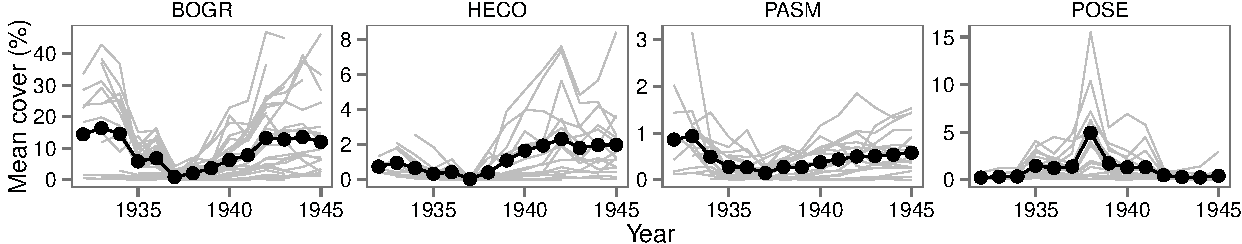
\includegraphics{components/figure/manuscript-figure_1-1.pdf}
\caption{Time series of average percent cover over all quadrats for our
four focal species: \emph{Bouteloua gracilis} (BOGR), \emph{Hesperostipa
comata} (HECO), \emph{Pascopyrum smithii} (PASM), and \emph{Poa secunda}
(POSE). Light grey lines show trajectories of individual quadrats. Note
the different y-axis scales across panels. See Table 1 for sample size
information.}
\end{figure}

\newpage{}

\begin{figure}[!ht]
  \centering
      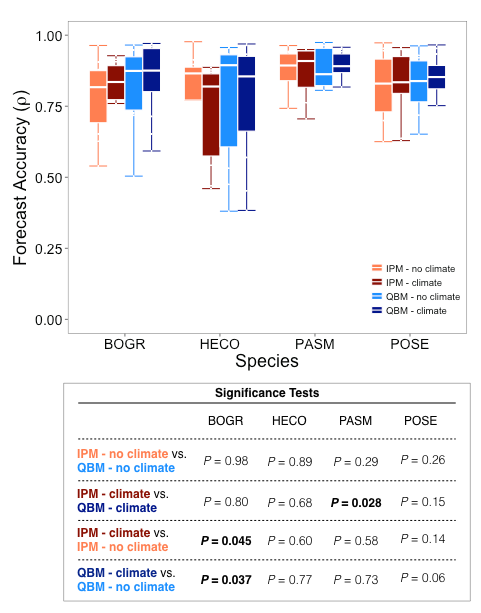
\includegraphics[height=6in]{./components/forecast_accuracy_mockup_boxplot.png}
  \caption{Comparisons of one-step-ahead, out-of-sample forecast accuracy between the IPM and QBM models with and without the inclusion of climate covariates. \textcolor{blue}{Boxplots show the distribution of $\rho$ averaged over quadrats for each cross-validation year (i.e., 13 values of $\rho$ for each species-model combination).} For each comparison, \emph{P}-values are from one-sided \emph{t} tests designed to assess whether the first model in the comparison statement had higher accuracy than the second model in the comparison statement (see details in Table S22). \textcolor{blue}{Statistical tests relied on correlation values for each quadrat-year-species combination, after averaging over model reps for each combination.} In no case did adding climate covariates decrease forecast accuracy (Table S21). Species codes are as in Fig. 1.}
\end{figure}

\newpage{}

\begin{figure}[!ht]
  \centering
      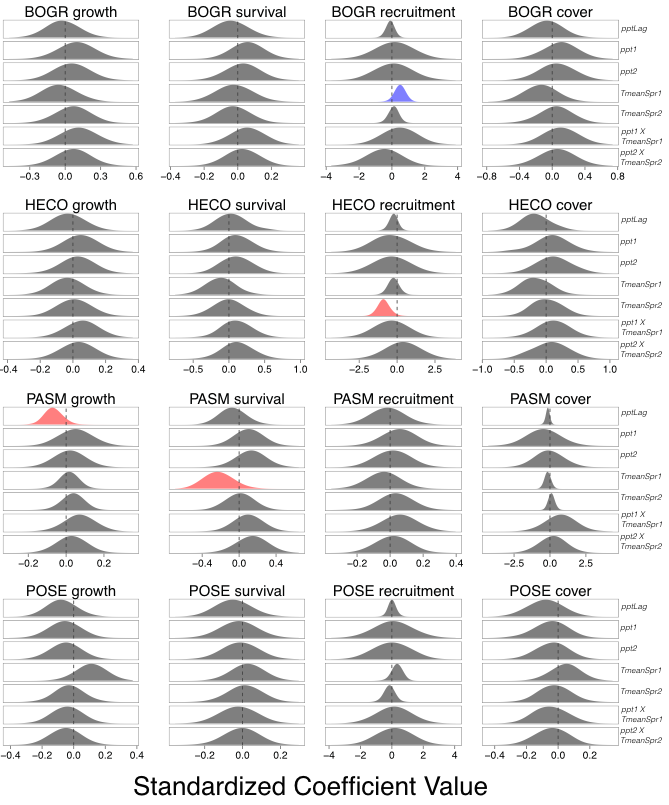
\includegraphics[height=7in]{./components/climate_posteriors_figure.png}
  \caption{Posterior distributions of climate effects ($\boldsymbol{\beta}_C$) for each species and vital rate statistical model. Because our priors were constrained via ridge-regression, we highlight climate effects whose 80\% credible intervals do not overlap zero (red for negative coefficients, blue for positive coefficients). Kernel bandwidths of posterior densities were adjusted by a factor of 4 for visual clarity. Species codes are as in Fig. 1. \textcolor{blue}{Climate covariate codes: \emph{pptLag} = "water year" precipitation at \emph{t}-2; \emph{ppt1} = April through June precipitation at \emph{t}-1; \emph{ppt2} = April through June precipitation at \emph{t}; \emph{TmeanSpr1} = April through June temperature at \emph{t}-1; \emph{TmeanSpr2} = April through June temperature at \emph{t}.}}
\end{figure}

\newpage{}

\begin{figure}[!ht]
  \centering
      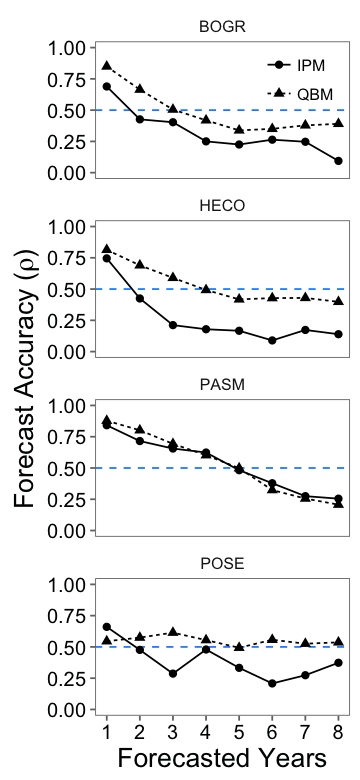
\includegraphics[height=5in]{./components/forecast_horizon.png}
  \caption{The forecast horizons for both models with climate covariates included \textcolor{blue}{and using mean parameter values. Points show the average accuracy ($\rho$, \textcolor{blue}{correlation between observations and predictions}) across all forecasts at a given distance between the last observation and the forecast, where forecasts are made for in-sample data.} We only examine the forecast accuracy of models with climate covariates included because in no case did including climate covariates significantly decrease accuracy (see Fig. 2). \textcolor{blue}{The dashed blue line indicates a forecast proficiency threshold of $\rho = 0.5$. Species codes are as in Fig. 1 and statistical comparisons between the IPM and QBM at each forecast distance are in Tables S23 and S24.}}
\end{figure}

\newpage{}

\singlespace{}

\subsection*{References}\label{references}
\addcontentsline{toc}{subsection}{References}

Adler, P. B., H. J. Dalgleish, and S. P. Ellner. 2012. Forecasting plant
community impacts of climate variability and change: when do competitive
interactions matter? Journal of Ecology 100:478--487.

Adler, P. B., S. P. Ellner, and J. M. Levine. 2010. Coexistence of
perennial plants: An embarrassment of niches. Ecology Letters
13:1019--1029.

Anderson, J., L. Vermeire, and P. B. Adler. 2011. Fourteen years of
mapped, permanent quadrats in a northern mixed prairie, USA. Ecology
92:1703.

Chu, C., and P. B. Adler. 2015. Large niche differences emerge at the
recruitment stage to stabilize grassland coexistence. Ecological
Monographs 85:373--392.

Chu, C., K. M. Havstad, N. Kaplan, W. K. Lauenroth, M. P. McClaran, D.
P. Peters, L. T. Vermeire, and P. B. Adler. 2014. Life form influences
survivorship patterns for 109 herbaceous perennials from six semi-arid
ecosystems. Journal of Vegetation Science 25:947--954.

Chu, C., A. R. Kleinhesselink, K. M. Havstad, M. P. McClaran, D. P.
Peters, L. T. Vermeire, H. Wei, and P. B. Adler. 2016. Direct effects
dominate responses to climate perturbations in grassland plant
communities. Nature Communications 7.

Clark, J. S., and O. N. Bj{ø}rnstad. 2004. Population time series:
Process variability, observation errors, missing values, lags, and
hidden states. Ecology 85:3140--3150.

Clark, J. S., D. M. Bell, M. H. Hersh, M. C. Kwit, E. Moran, C. Salk, A.
Stine, D. Valle, and K. Zhu. 2011. Individual-scale variation,
species-scale differences: Inference needed to understand diversity.
Ecology Letters 14:1273--1287.

Clark, J. S., D. M. Bell, M. Kwit, A. Stine, B. Vierra, and K. Zhu.
2012. Individual-scale inference to anticipate climate-change
vulnerability of biodiversity. Philosophical Transactions of the Royal
Society B: Biological Sciences 367:236--246.

Clark, J. S., D. Bell, C. Chu, B. Courbaud, M. Dietze, M. Hersh, J.
HilleRisLambers, I. Ib{á}{ñ}ez, S. LaDeau, S. McMahon, J. Metcalf, J.
Mohan, E. Moran, L. Pangle, S. Pearson, C. Salk, Z. Shen, D. Valle, and
P. Wyckoff. 2010. High-dimensional coexistence based on individual
variation: a synthesis of evidence. Ecological Monographs 80:569--608.

Clark, J. S., S. R. Carpenter, M. Barber, S. Collins, A. Dobson, J. A.
Foley, D. M. Lodge, M. Pascual, R. Pielke, W. Pizer, C. Pringle, W. V.
Reid, K. A. Rose, O. Sala, W. H. Schlesinger, D. H. Wall, and D. Wear.
2001. Ecological forecasts: an emerging imperative. Science (New York,
N.Y.) 293:657--660.

Cribari-Neto, F. 2004. Asymptotic inference under heteroskedasticity of
unknown form. Computational Statistics and Data Analysis 45:215--233.

Dalgleish, H. J., D. N. Koons, M. B. Hooten, C. A. Moffet, and P. B.
Adler. 2011. Climate influences the demography of three dominant
sagebrush steppe plants. Ecology 92:75--85.

Ellner, S. P., and M. Rees. 2006. Integral projection models for species
with complex demography. The American naturalist 167:410--428.

Evans, M. R. 2012. Modelling ecological systems in a changing world.
Philosophical transactions of the Royal Society of London. Series B,
Biological sciences 367:181--190.

Freckleton, R. P., W. J. Sutherland, A. R. Watkinson, and S. A.
Queenborough. 2011. Density-structured models for plant population
dynamics. American Naturalist 177:1--17.

Gelman, A., J. Hwang, and A. Vehtari. 2014. Understanding predictive
information criteria for Bayesian models. Statistics and Computing
24:997--1016.

Gerber, B. D., W. L. Kendall, M. B. Hooten, J. A. Dubovsky, and R. C.
Drewien. 2015. Optimal population prediction of sandhill crane
recruitment based on climate-mediated habitat limitations. Journal of
Animal Ecology 84:1299--1310.

Hobbs, N. T., and M. B. Hooten. 2015. Bayesian Models: A Statistical
Primer for Ecologists. Princeton University Press, Princeton.

Hooten, M. B., and N. T. Hobbs. 2015. A guide to Bayesian model
selection for ecologists. Ecological Monographs 85:3--28.

Lauenroth, W. K., and P. B. Adler. 2008. Demography of perennial
grassland plants: Survival, life expectancy and life span. Journal of
Ecology 96:1023--1032.

Luo, Y., K. Ogle, C. Tucker, S. Fei, C. Gao, S. LaDeau, J. S. Clark, and
D. S. Schimel. 2011. Ecological forecasting and data assimilation in a
data-rich era. Ecological Applications 21:1429--1442.

Mouquet, N., Y. Lagadeuc, V. Devictor, L. Doyen, A. Duputi{é}, D.
Eveillard, D. Faure, E. Garnier, O. Gimenez, P. Huneman, F. Jabot, P.
Jarne, D. Joly, R. Julliard, S. K{é}fi, G. J. Kergoat, S. Lavorel, L.
{Le Gall}, L. Meslin, S. Morand, X. Morin, H. Morlon, G. Pinay, R.
Pradel, F. M. Schurr, W. Thuiller, and M. Loreau. 2015. Predictive
ecology in a changing world.

Perretti, C. T., S. B. Munch, and G. Sugihara. 2013. Model-free
forecasting outperforms the correct mechanistic model for simulated and
experimental data. Proceedings of the National Academy of Sciences of
the United States of America 110:5253--5257.

Petchey, O. L., M. Pontarp, T. M. Massie, S. K{é}fi, A. Ozgul, M.
Weilenmann, G. M. Palamara, F. Altermatt, B. Matthews, J. M. Levine, D.
Z. Childs, B. J. McGill, M. E. Schaepman, B. Schmid, P. Spaak, A. P.
Beckerman, F. Pennekamp, and I. S. Pearse. 2015. The ecological forecast
horizon, and examples of its uses and determinants. Ecology Letters
18:597--611.

Pol, M. van de, and A. Cockburn. 2011. Identifying the critical climatic
time window that affects trait expression. The American naturalist
177:698--707.

Queenborough, S. A., K. M. Burnet, W. J. Sutherland, A. R. Watkinson,
and R. P. Freckleton. 2011. From meso- to macroscale population
dynamics: A new density-structured approach. Methods in Ecology and
Evolution 2:289--302.

R Core Team. 2013. R: A language and environment for statistical
computing.

Rees, M., and S. P. Ellner. 2009. Integral projection models for
populations in temporally varying environments. Ecological Monographs
79:575--594.

Schindler, D. E., and R. Hilborn. 2015. Prediction, precaution, and
policy under global change. Science 347:953--954.

Sims, M., D. A. Elston, A. Larkham, D. H. Nussey, and S. D. Albon. 2007.
Identifying when weather influences life-history traits of grazing
herbivores. Journal of Animal Ecology 76:761--770.

Stan Development Team. 2014a. Stan: A C++ Library for Probability and
Sampling, Version 2.5.0.

Stan Development Team. 2014b. Rstan: the R interface to Stan, Version
2.5.0.

S{æ}ther, B. E., S. Engen, V. Gr{ø}tan, W. Fiedler, E. Matthysen, M. E.
Visser, J. Wright, A. P. M{ø}ller, F. Adriaensen, H. {Van Balen}, D.
Balmer, M. C. Mainwaring, R. H. McCleery, M. Pampus, and W. Winkel.
2007. The extended Moran effect and large-scale synchronous fluctuations
in the size of great tit and blue tit populations. Journal of Animal
Ecology 76:315--325.

Taylor, C. M., and A. Hastings. 2004. Finding optimal control strategies
for invasive species: a density-structured model for Spartina
alterniflora. Journal of Applied Ecology 41:1049--1057.

Teller, B. J., P. B. Adler, C. B. Edwards, G. Hooker, R. E. Snyder, and
S. P. Ellner. 2016. Linking demography with drivers: climate and
competition. Methods in Ecology and Evolution 7:171--183.

Vehtari, A., A. Gelman, and J. Gabry. 2016. Efficient implementation of
leave-one-out cross-validation and WAIC for evaluating fitted Bayesian
models. ArXiv preprint.

Wilcox, R. R. 2009. Comparing Pearson Correlations: Dealing with
Heteroscedasticity and Nonnormality. Communications in Statistics -
Simulation and Computation 38:2220--2234.

Ye, H., R. J. Beamish, S. M. Glaser, S. C. H. Grant, C.-h. Hsieh, L. J.
Richards, J. T. Schnute, and G. Sugihara. 2015. Equation-free
mechanistic ecosystem forecasting using empirical dynamic modeling.
Proceedings of the National Academy of Sciences 112:E1569--E1576.

\end{document}
